\documentclass[10pt]{beamer}
\usepackage[utf8]{inputenc}
\usepackage[T1]{fontenc}
\usepackage[russian]{babel}
\usepackage{graphicx}
\usepackage{tikz}
\usepackage{pifont}
\usecolortheme{orchid}
\renewcommand{\familydefault}{verdana}
\setbeamerfont{block title}{size=\normalsize}
\title[World development indicators]{\huge World development indicators}
\subtitle[Which country will develop more]{\large Which country will develop more}
\author[Moawad, Commandi, Isaeva, Schiavon, Snesarevskii] {{\Large Group 12:\\}Stefano Moawad\\Leonardo Comandini\\Diana Isaeva\\Andrea Schiavon\\Viktor Snesarevskii}
\date{April-May 2017}
\usebackgroundtemplate{\tikz\node[opacity=0.3] {\vbox to \paperheight{\vfil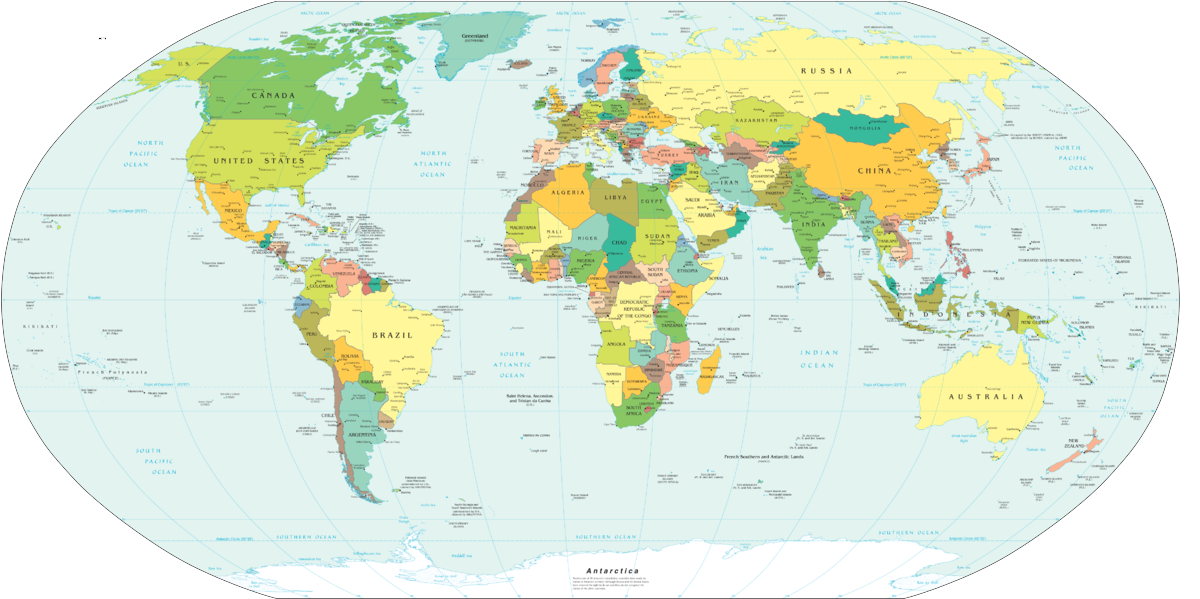
\includegraphics[width=\paperwidth]{map}\vfil}};}

\begin{document}
\begin{frame}
\titlepage
\vfill
\begin{flushright}

\includegraphics[height=.7cm]{kaggle.png}\quad

\includegraphics[height=.7cm]{worldbank.jpg}
\end{flushright}
\end{frame}

% snapshot raw dataset
\begin{frame}{Raw dataset}
\begin{block}{Indicators (6 columns)}
\scriptsize
\begin{tabular}{*{6}{l}}
Country name &
\only<1-1>{Country code}\only<2->{\!\!\tikz[baseline]\node[anchor=base,draw=red]{Country code};}& 
\!\! Indicator name & \!\! Indicator code & Year & 
\only<1-1>{Value}\only<2->{\!\!\tikz[baseline]\node[anchor=base,draw=cyan]{Value};}
\end{tabular}
\end{block}
\begin{block}{Country (31 columns)}
\scriptsize
\begin{tabular}{*{5}{l}}
\only<1-1>{Country code}\only<2->{\!\!\tikz[baseline]\node[anchor=base,draw=red]{Country code};}& 
Short name & Table name & Long name & Alpha 2 code \\[.15cm]
Currency unit & Special notes &
\only<1-1>{Region}\only<2->{\!\!\tikz[baseline]\node[anchor=base,draw=green]{Region};}&
Indice group & \textbf{etc...}
\end{tabular}
\end{block}

\begin{block}{Country notes (3 columns)}
\scriptsize
\begin{tabular}{*{5}{l}}
\only<1-1>{Country code}\only<2->{\!\!\tikz[baseline]\node[anchor=base,draw=red]{Country code};}&
\only<1-1>{Series code}\only<2->{\!\!\tikz[baseline]\node[anchor=base,draw=blue]{Series code};}&
Description
\end{tabular}
\end{block}
\begin{block}{Series (20 columns)}
\scriptsize
\begin{tabular}{*{4}{l}}
\only<1-1>{Series code}\only<2->{\!\!\tikz[baseline]\node[anchor=base,draw=blue]{Series code};}&
Topic & Indicator name\!\! & Short definition \\[.15cm] Long definition & 
\only<1-1>{Unit of measure}\only<2->{\!\!\tikz[baseline]\node[anchor=base,draw=orange]{Unit of measure};}&
Periodicity  & \textbf{etc...}
\end{tabular}
\end{block}
\begin{block}{Series notes (3 columns)}
\scriptsize
\begin{tabular}{*{5}{l}}
\only<1-1>{Series code}\only<2->{\!\!\tikz[baseline]\node[anchor=base,draw=blue]{Series code};}&
\only<1-1>{Year}\only<2->{\!\!\tikz[baseline]\node[anchor=base,draw=black]{Year};}&
Description
\end{tabular}
\end{block}
\end{frame}

\begin{frame}{Examples of indicators}
	\begin{figure}
		\centering
		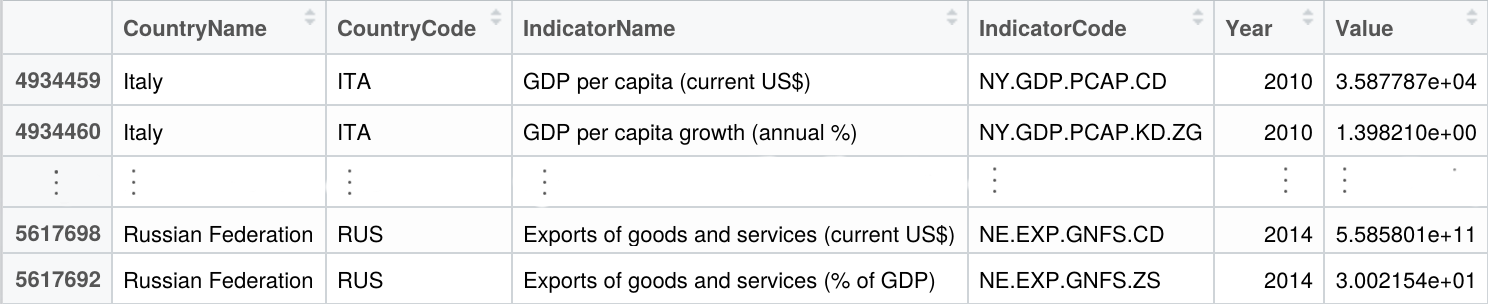
\includegraphics [width=\textwidth]{indicators.png}
		
	\end{figure}
\end{frame}


\begin{frame}
	\begin{figure}
		\centering
		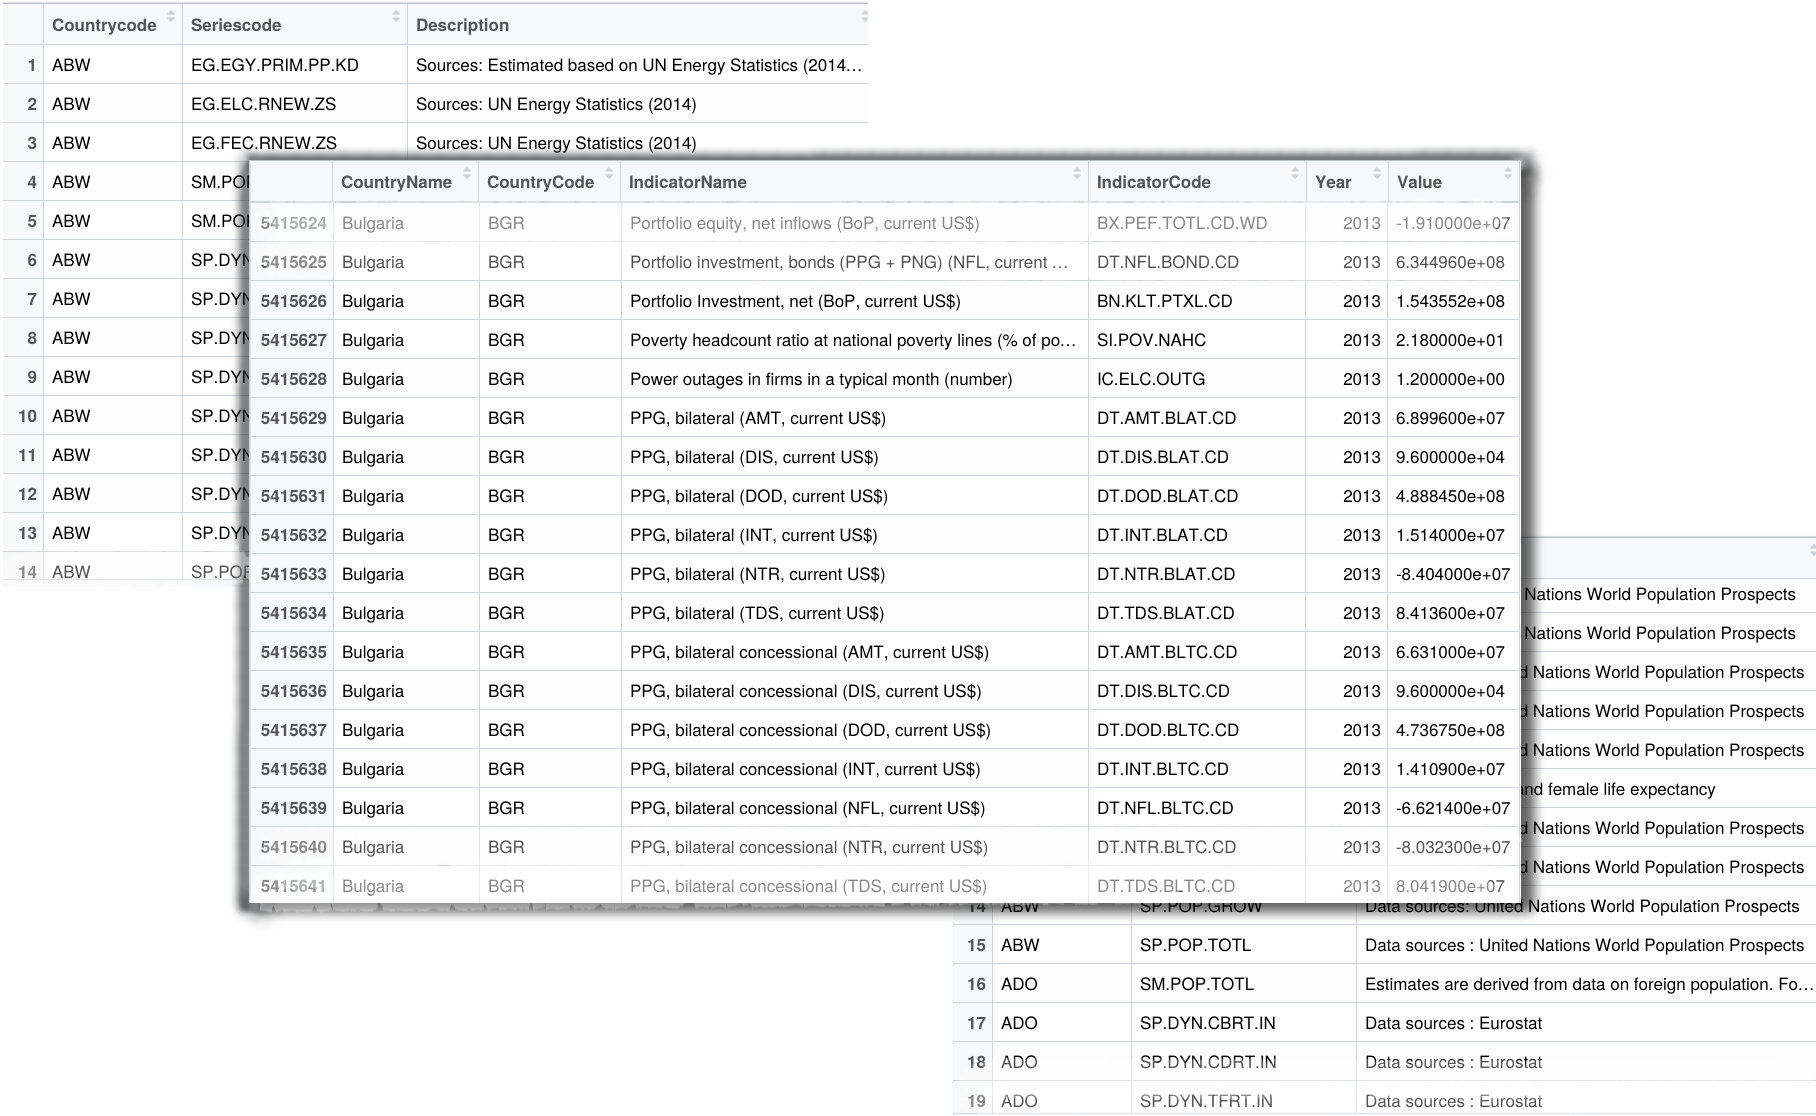
\includegraphics[width=\textwidth]{tables_2.png}
	\end{figure}
\end{frame}

\begin{frame}
	Looking at \textit{Indicators} as a 3D matrix leads to some problems
	\begin{itemize}
		\item YEARS \ding{221} not homogeneous
		\item COUNTRIES \ding{221} small ones
		\item INDICATORS \ding{221} too many to choose easily
	\end{itemize}
\end{frame}

\begin{frame}
	\begin{figure}
		\centering
		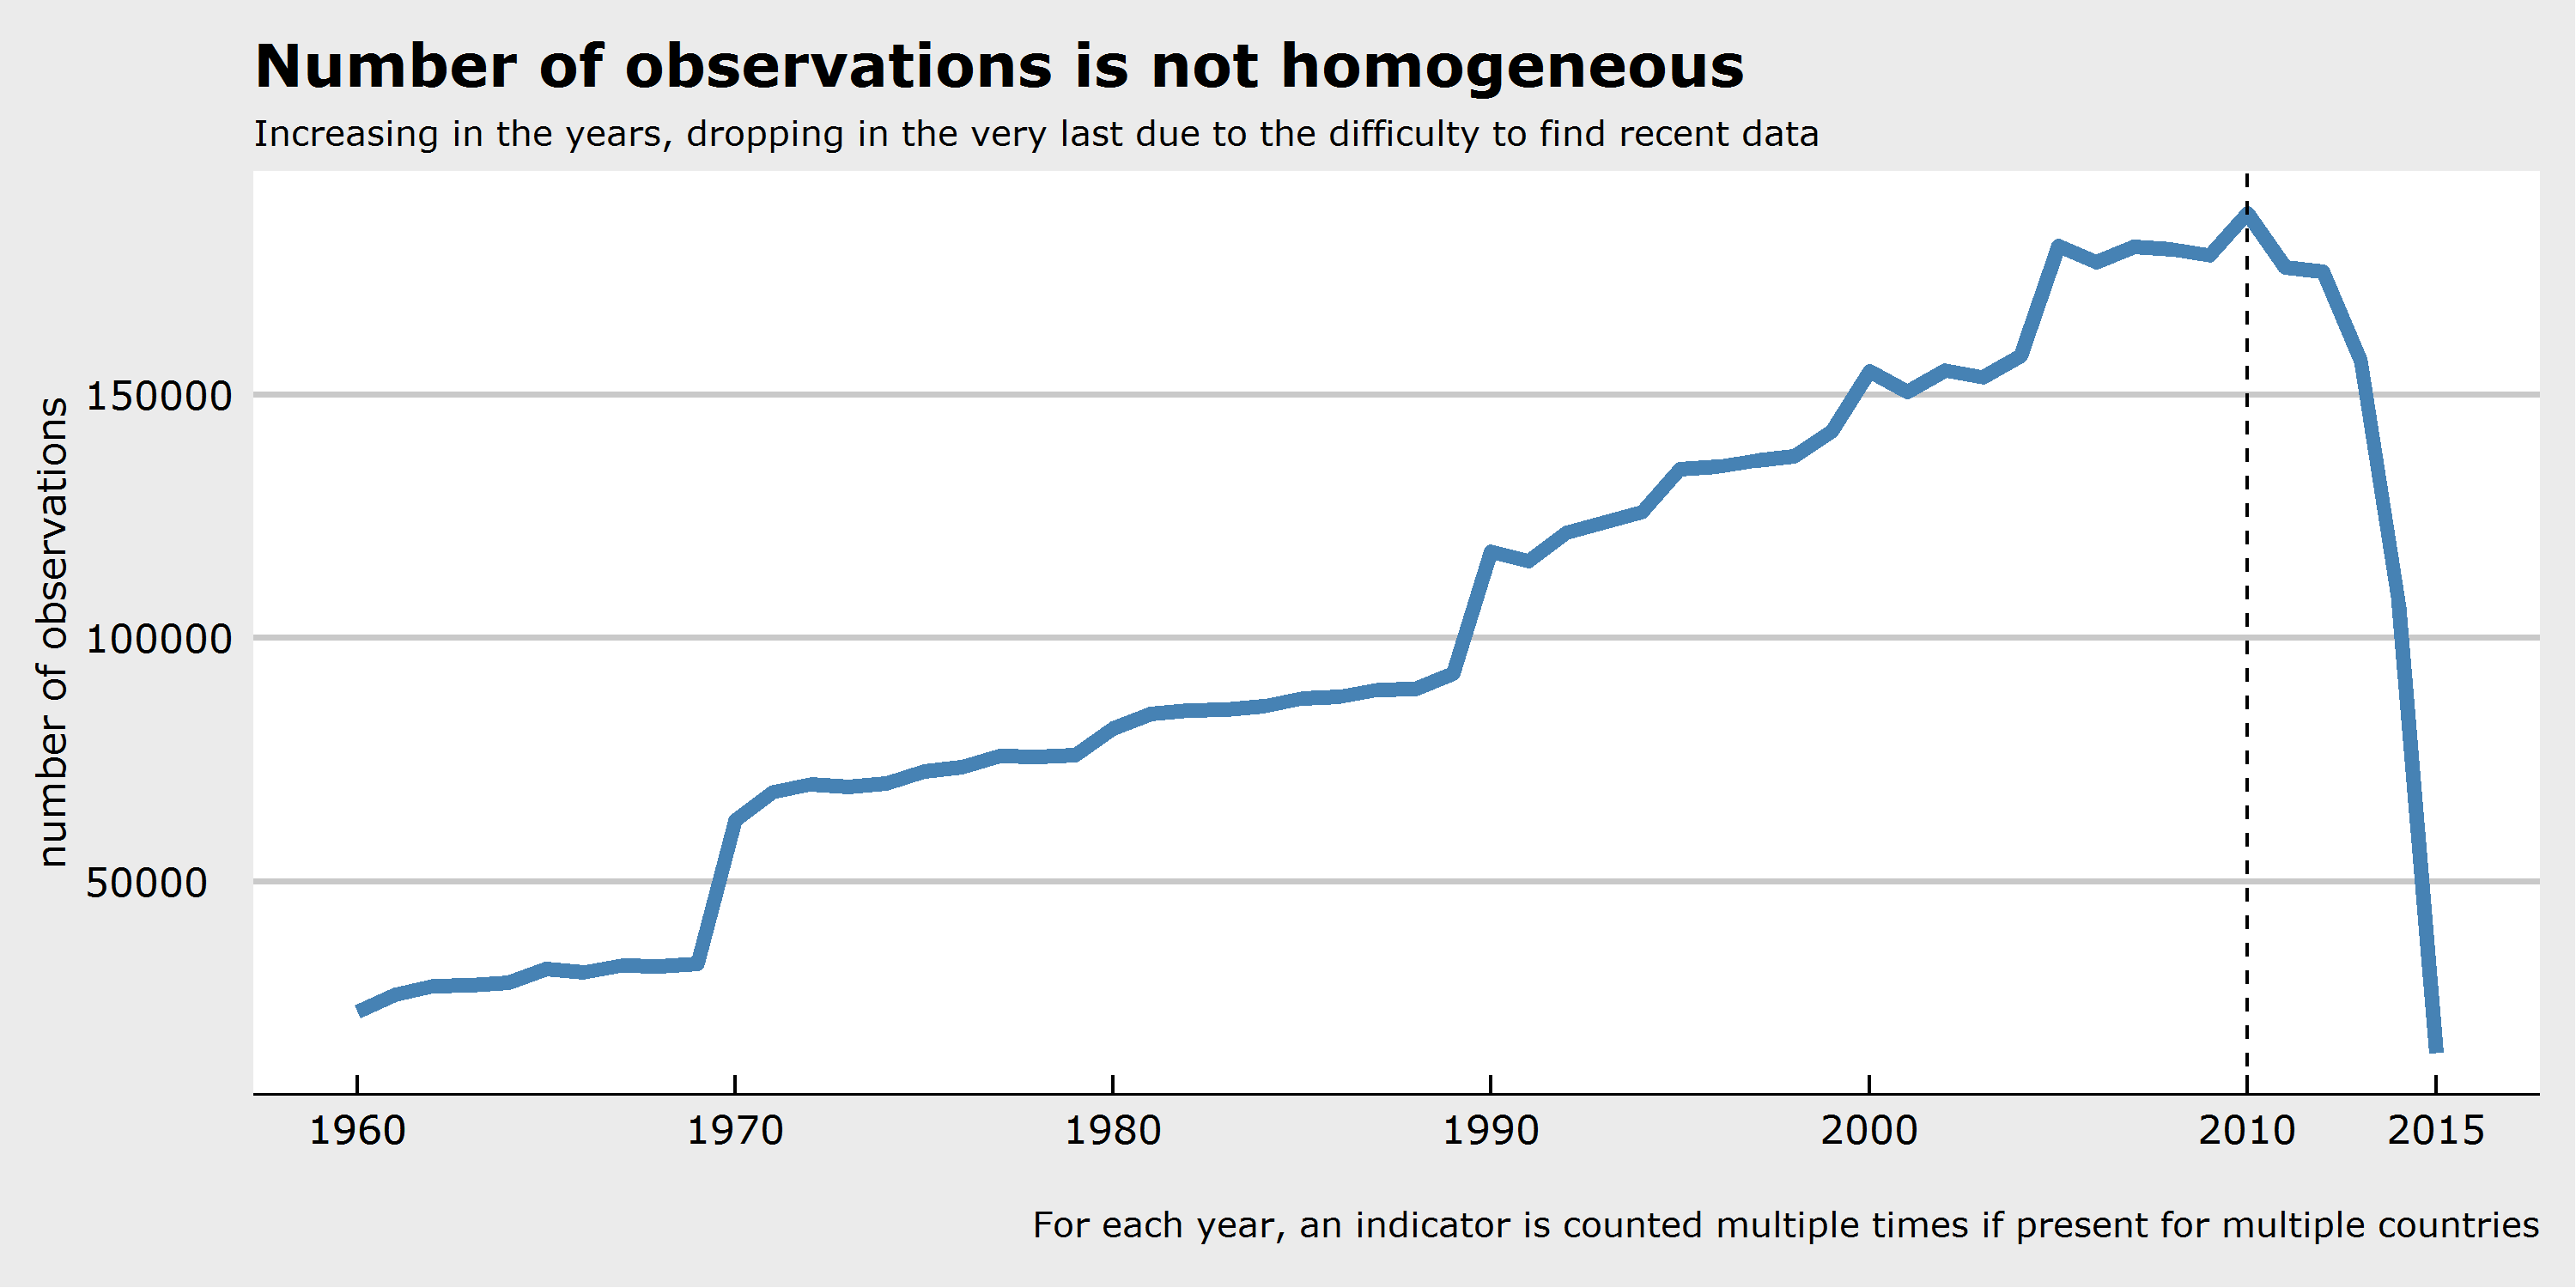
\includegraphics[width=\textwidth]{plot0001.png}
	\end{figure}
\end{frame}

\begin{frame}
	\begin{figure}
		\centering
		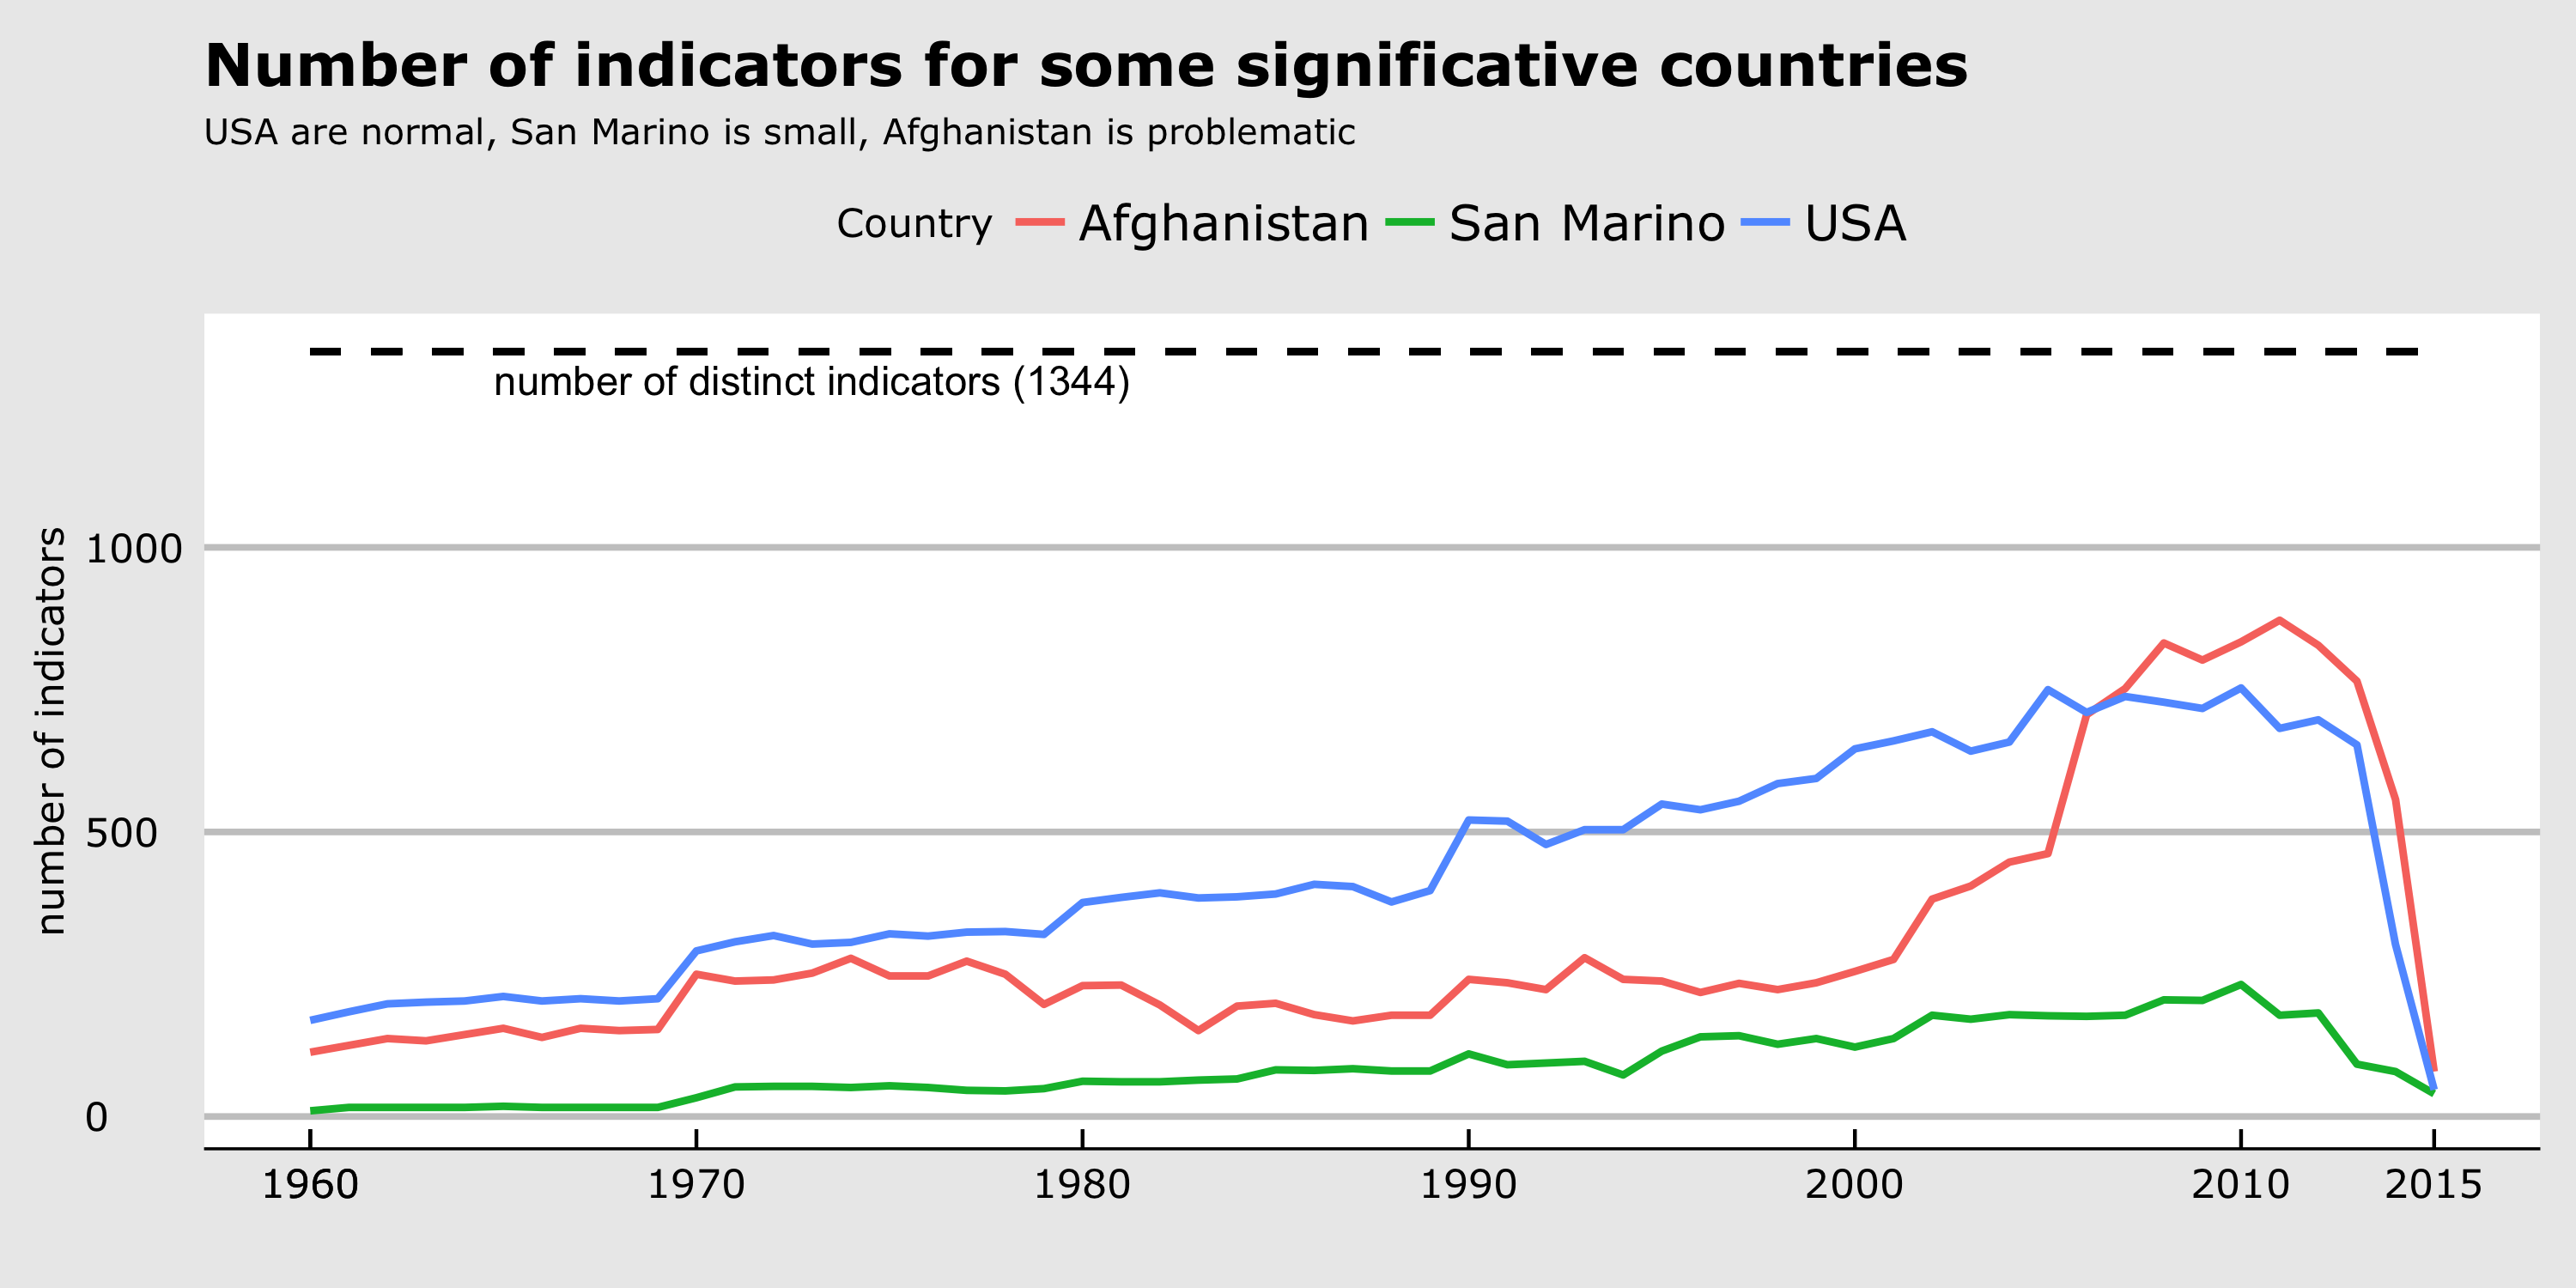
\includegraphics[width=\textwidth]{plot0002.png}
	\end{figure}
\end{frame}

\begin{frame}
	\begin{figure}
		\centering
		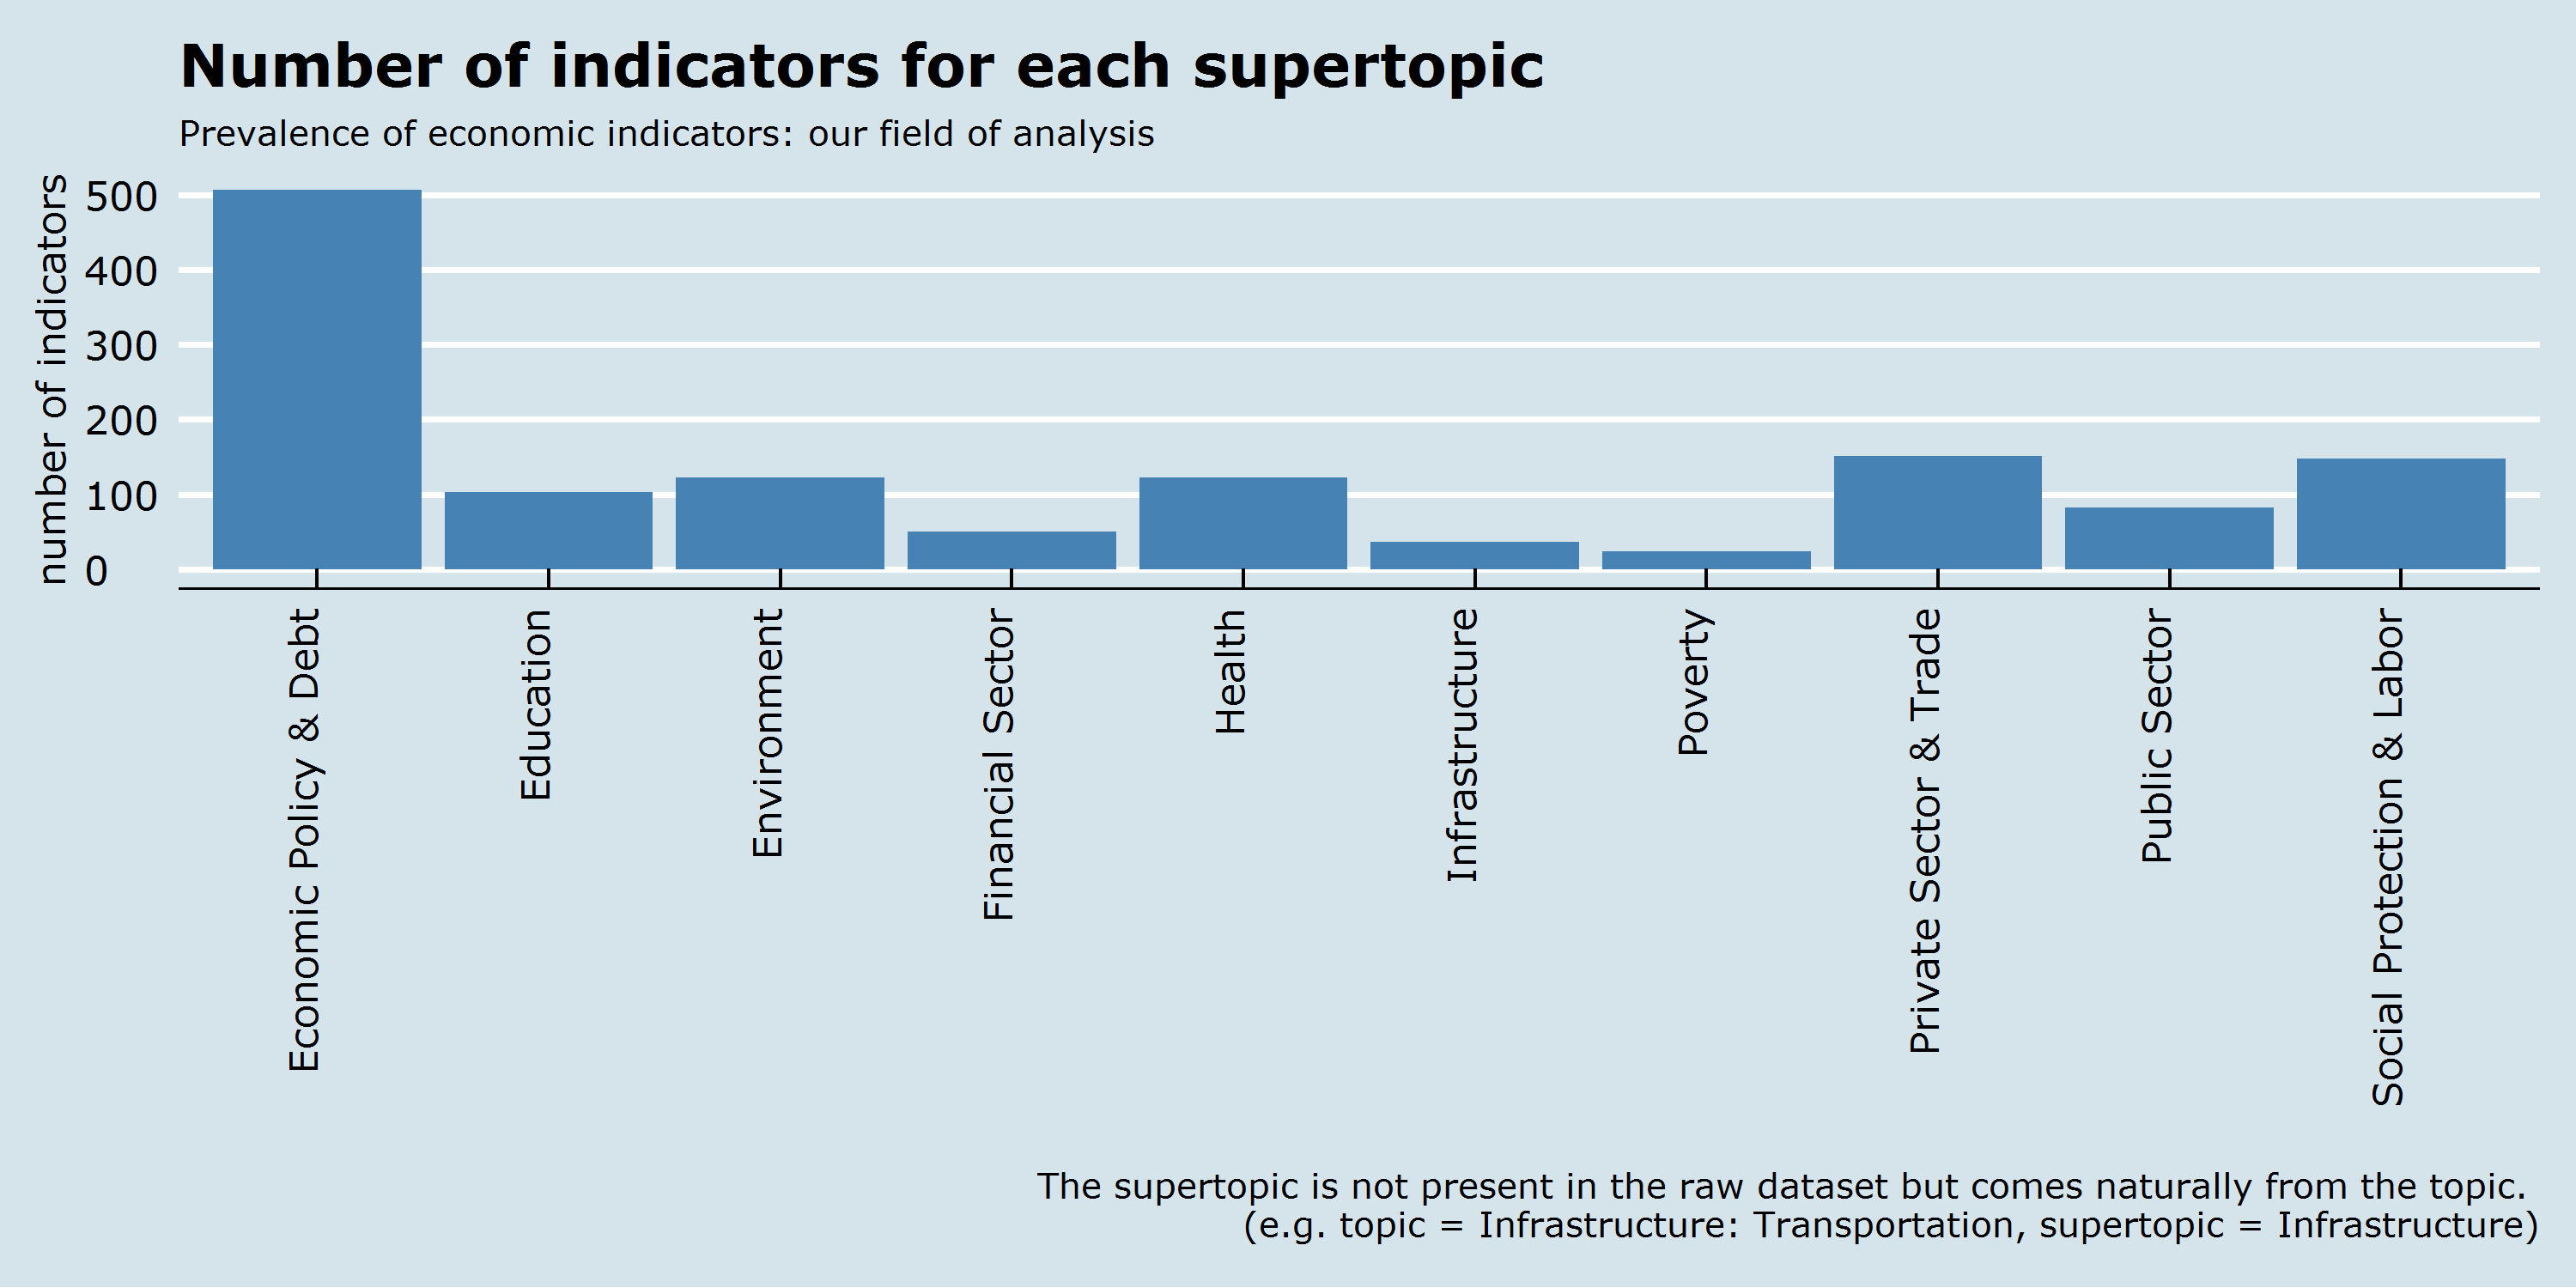
\includegraphics[width=\textwidth]{plot0003.png}
	\end{figure}
\end{frame}

\begin{frame}
	\begin{figure}
		\centering
		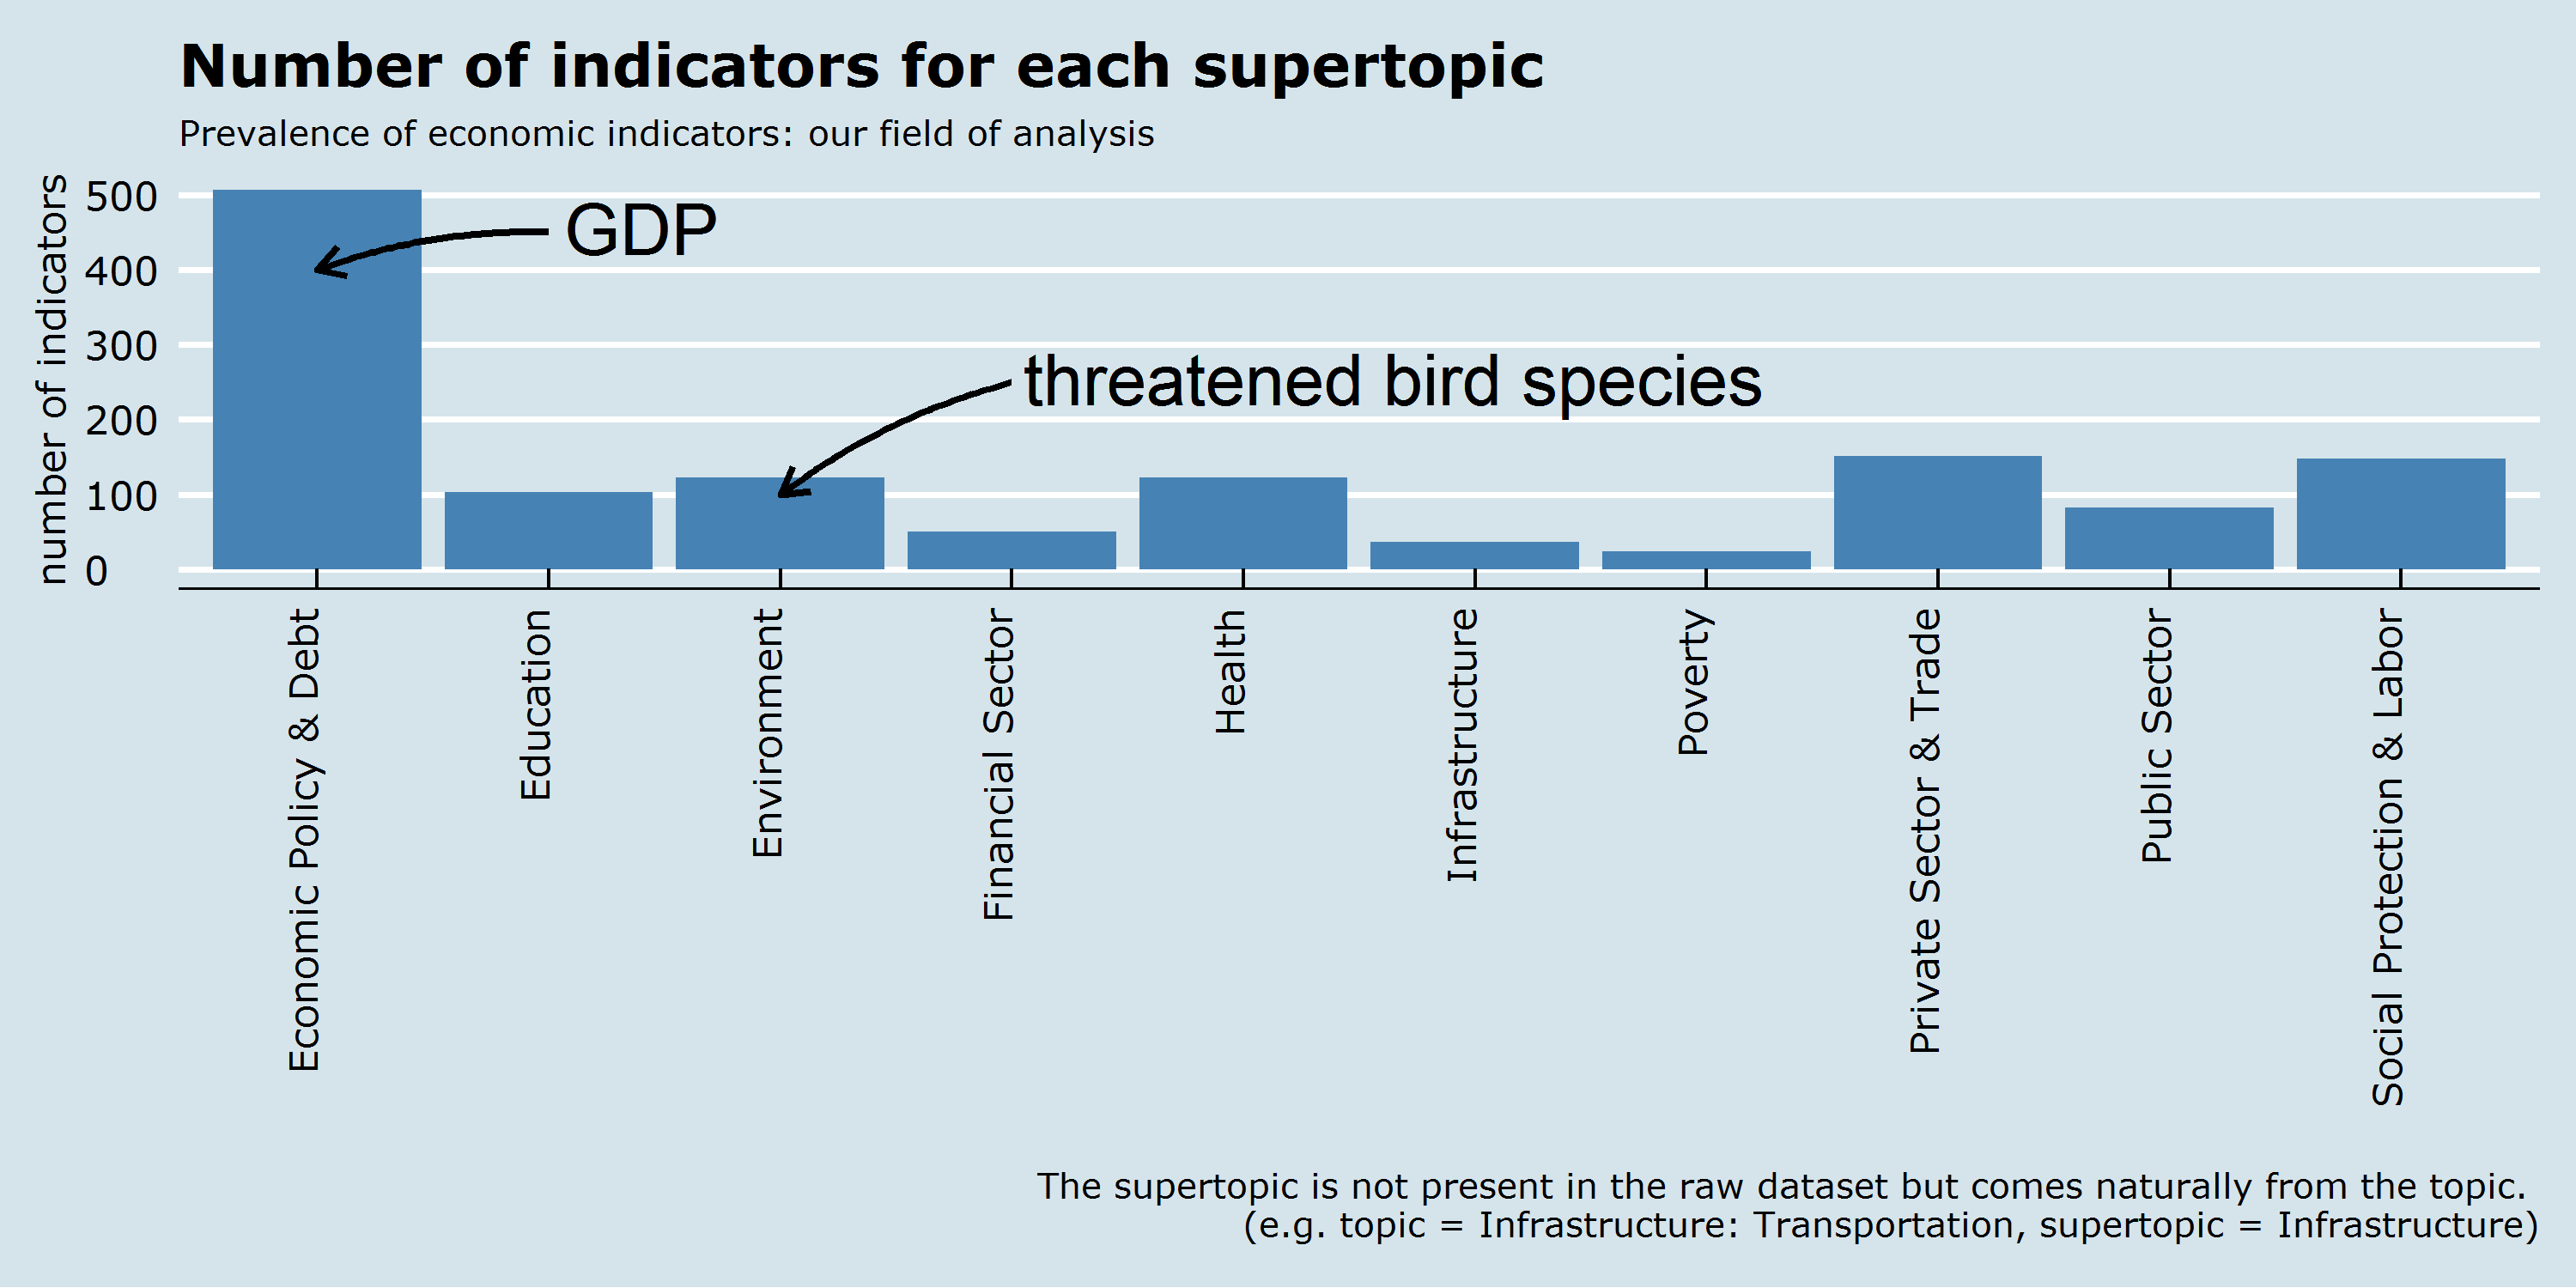
\includegraphics[width=\textwidth]{plot0004.png}
	\end{figure}
\end{frame}

\begin{frame}
	\begin{center}
		{\Large An intermediate goal:} \\[.2cm]
		Extract a full matrix with meaningful indicators to perform PCA
	\end{center}
\end{frame}

\begin{frame}
	\begin{center}
		{\Large Fix the best year: \\[.3cm]
		2010}
	\end{center}
\end{frame}

\begin{frame}
	\begin{figure}
		\centering
		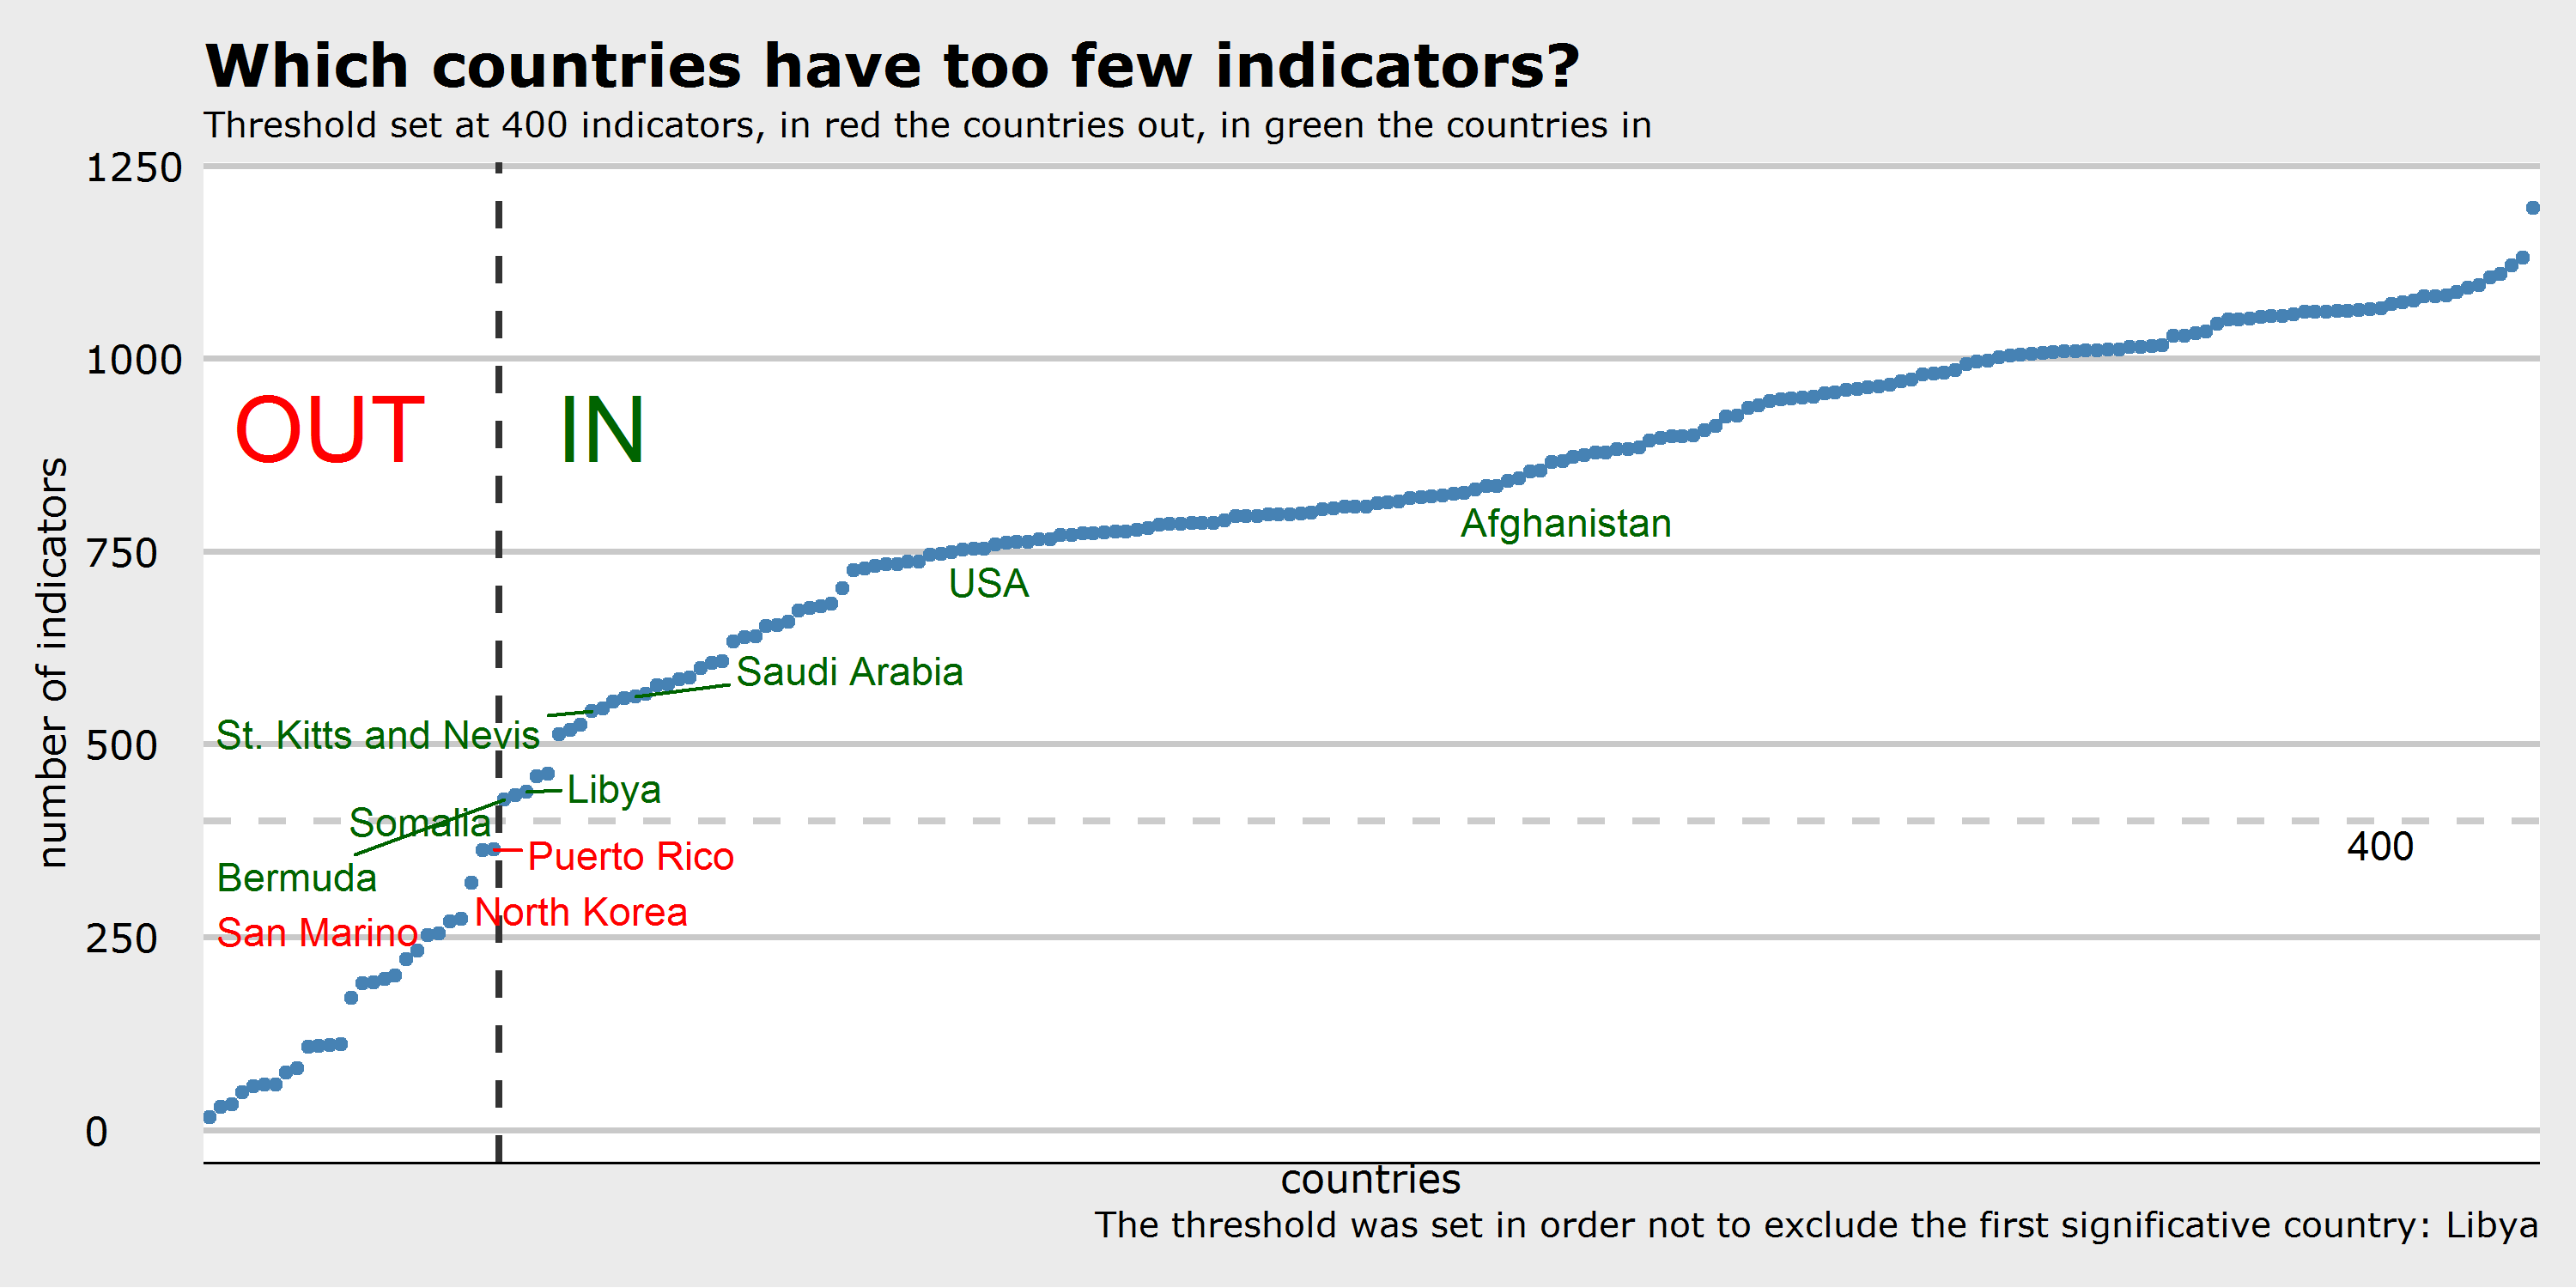
\includegraphics[width=\textwidth]{plot0005.png}
	\end{figure}
\end{frame}

\begin{frame}
	\begin{figure}
		\centering
		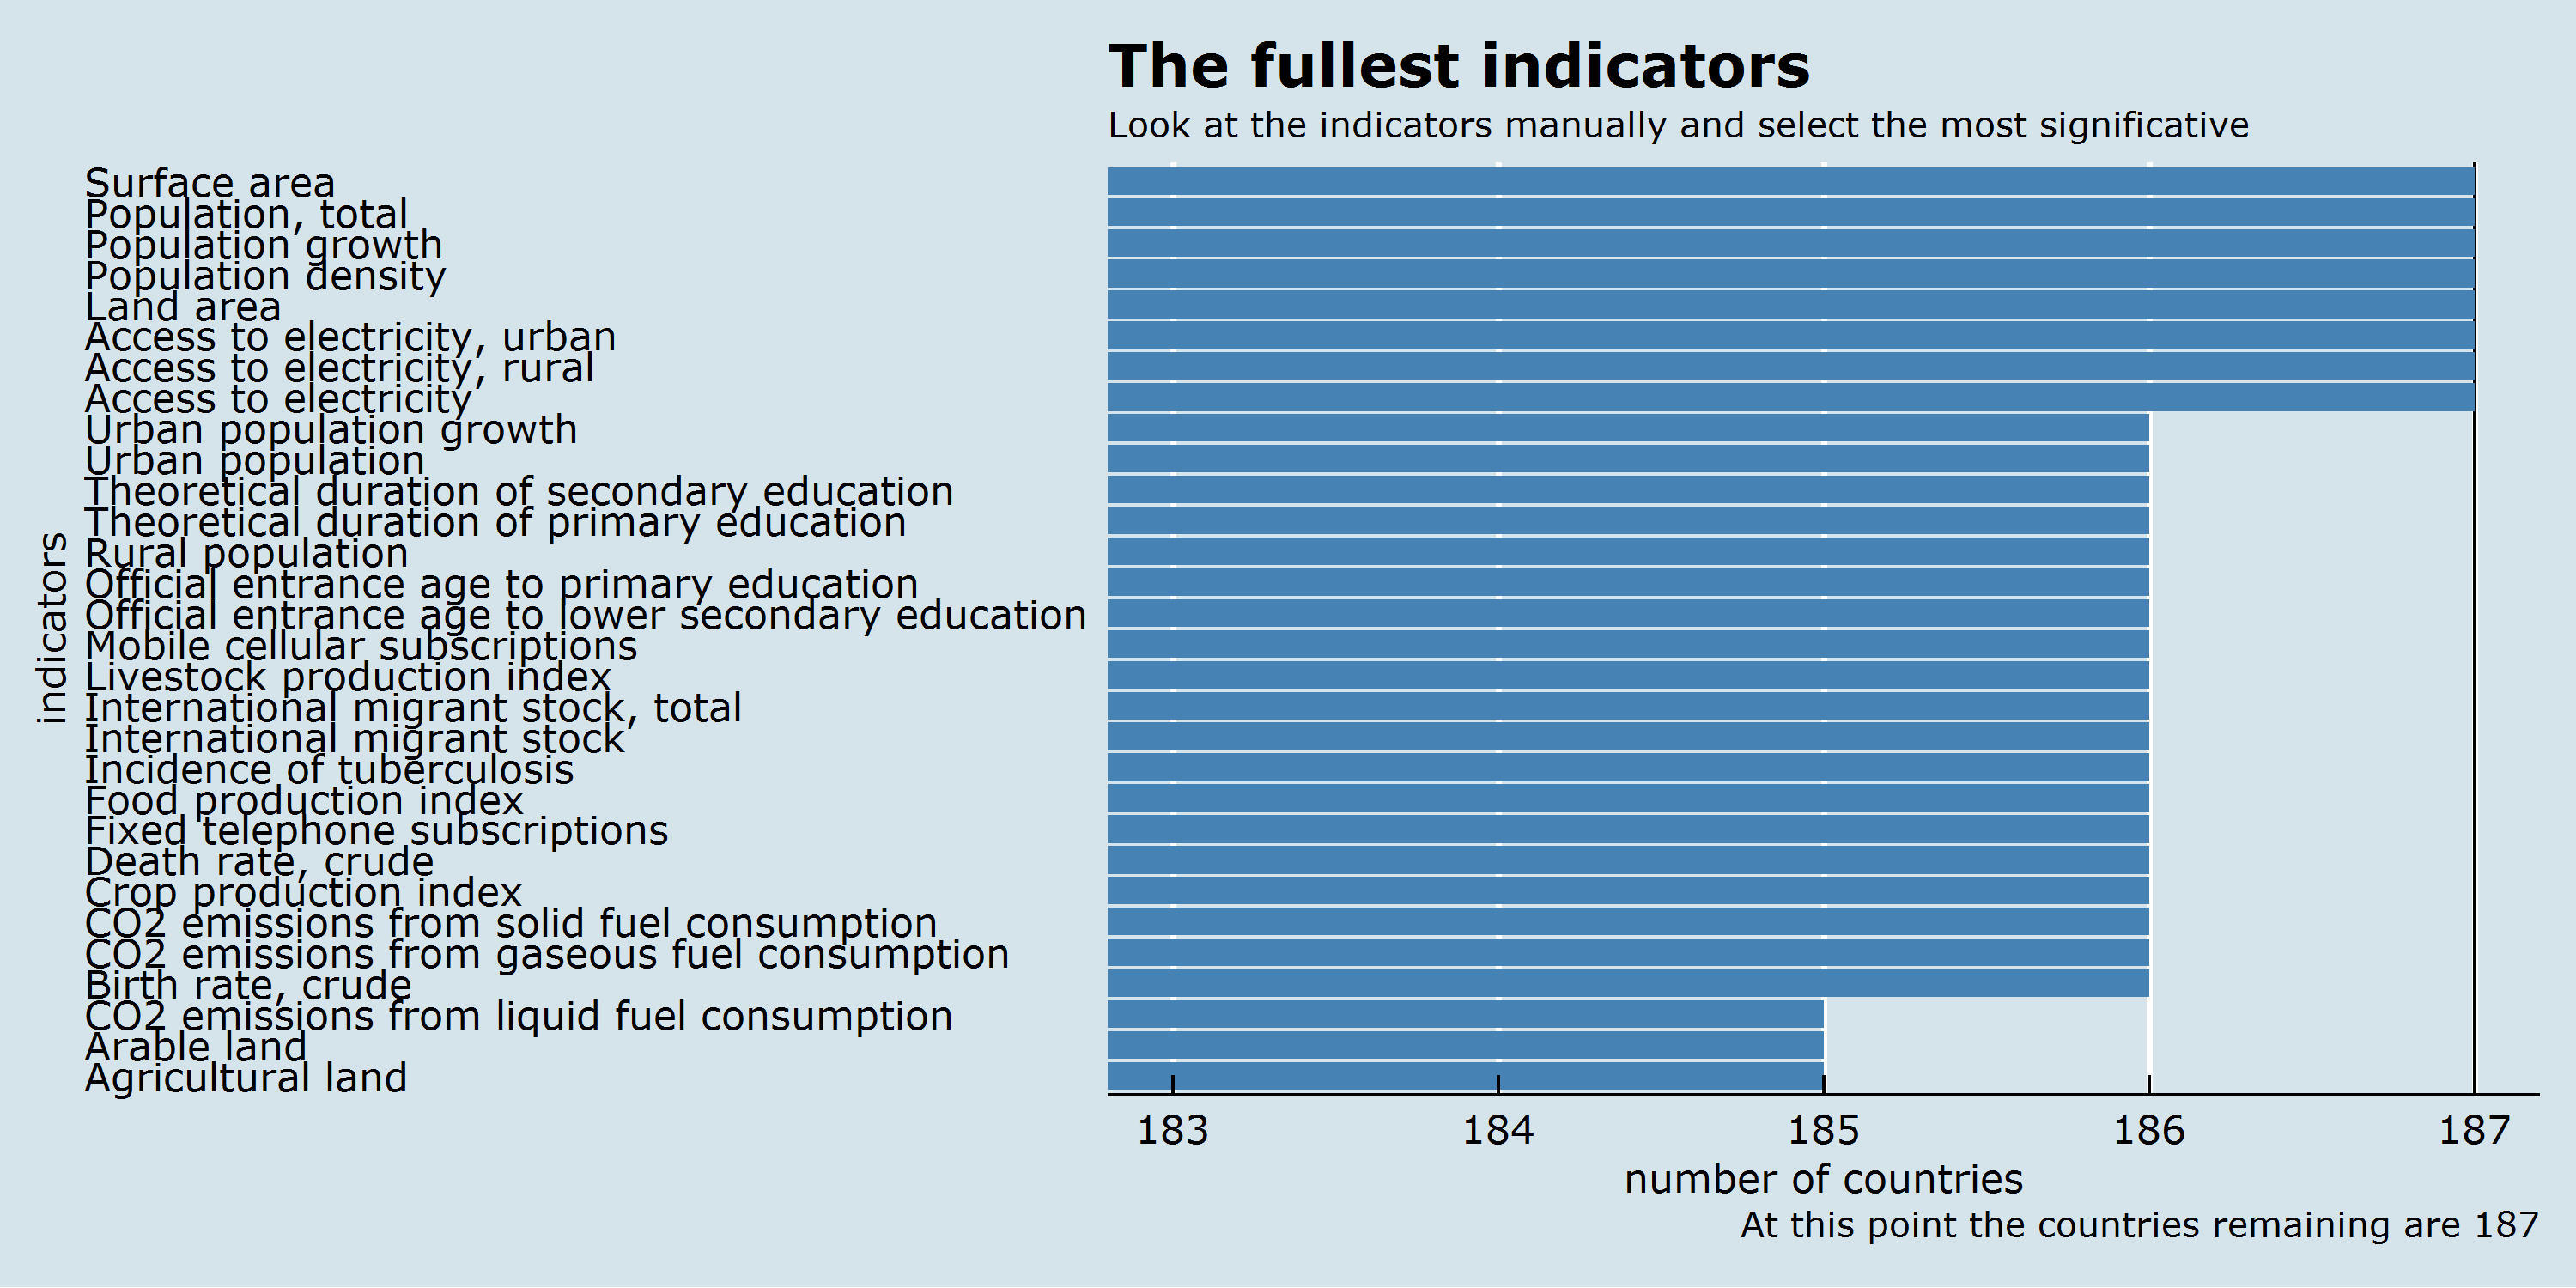
\includegraphics[width=\textwidth]{plot0006.png}
	\end{figure}
\end{frame}

\begin{frame}
	\begin{figure}
		\centering
		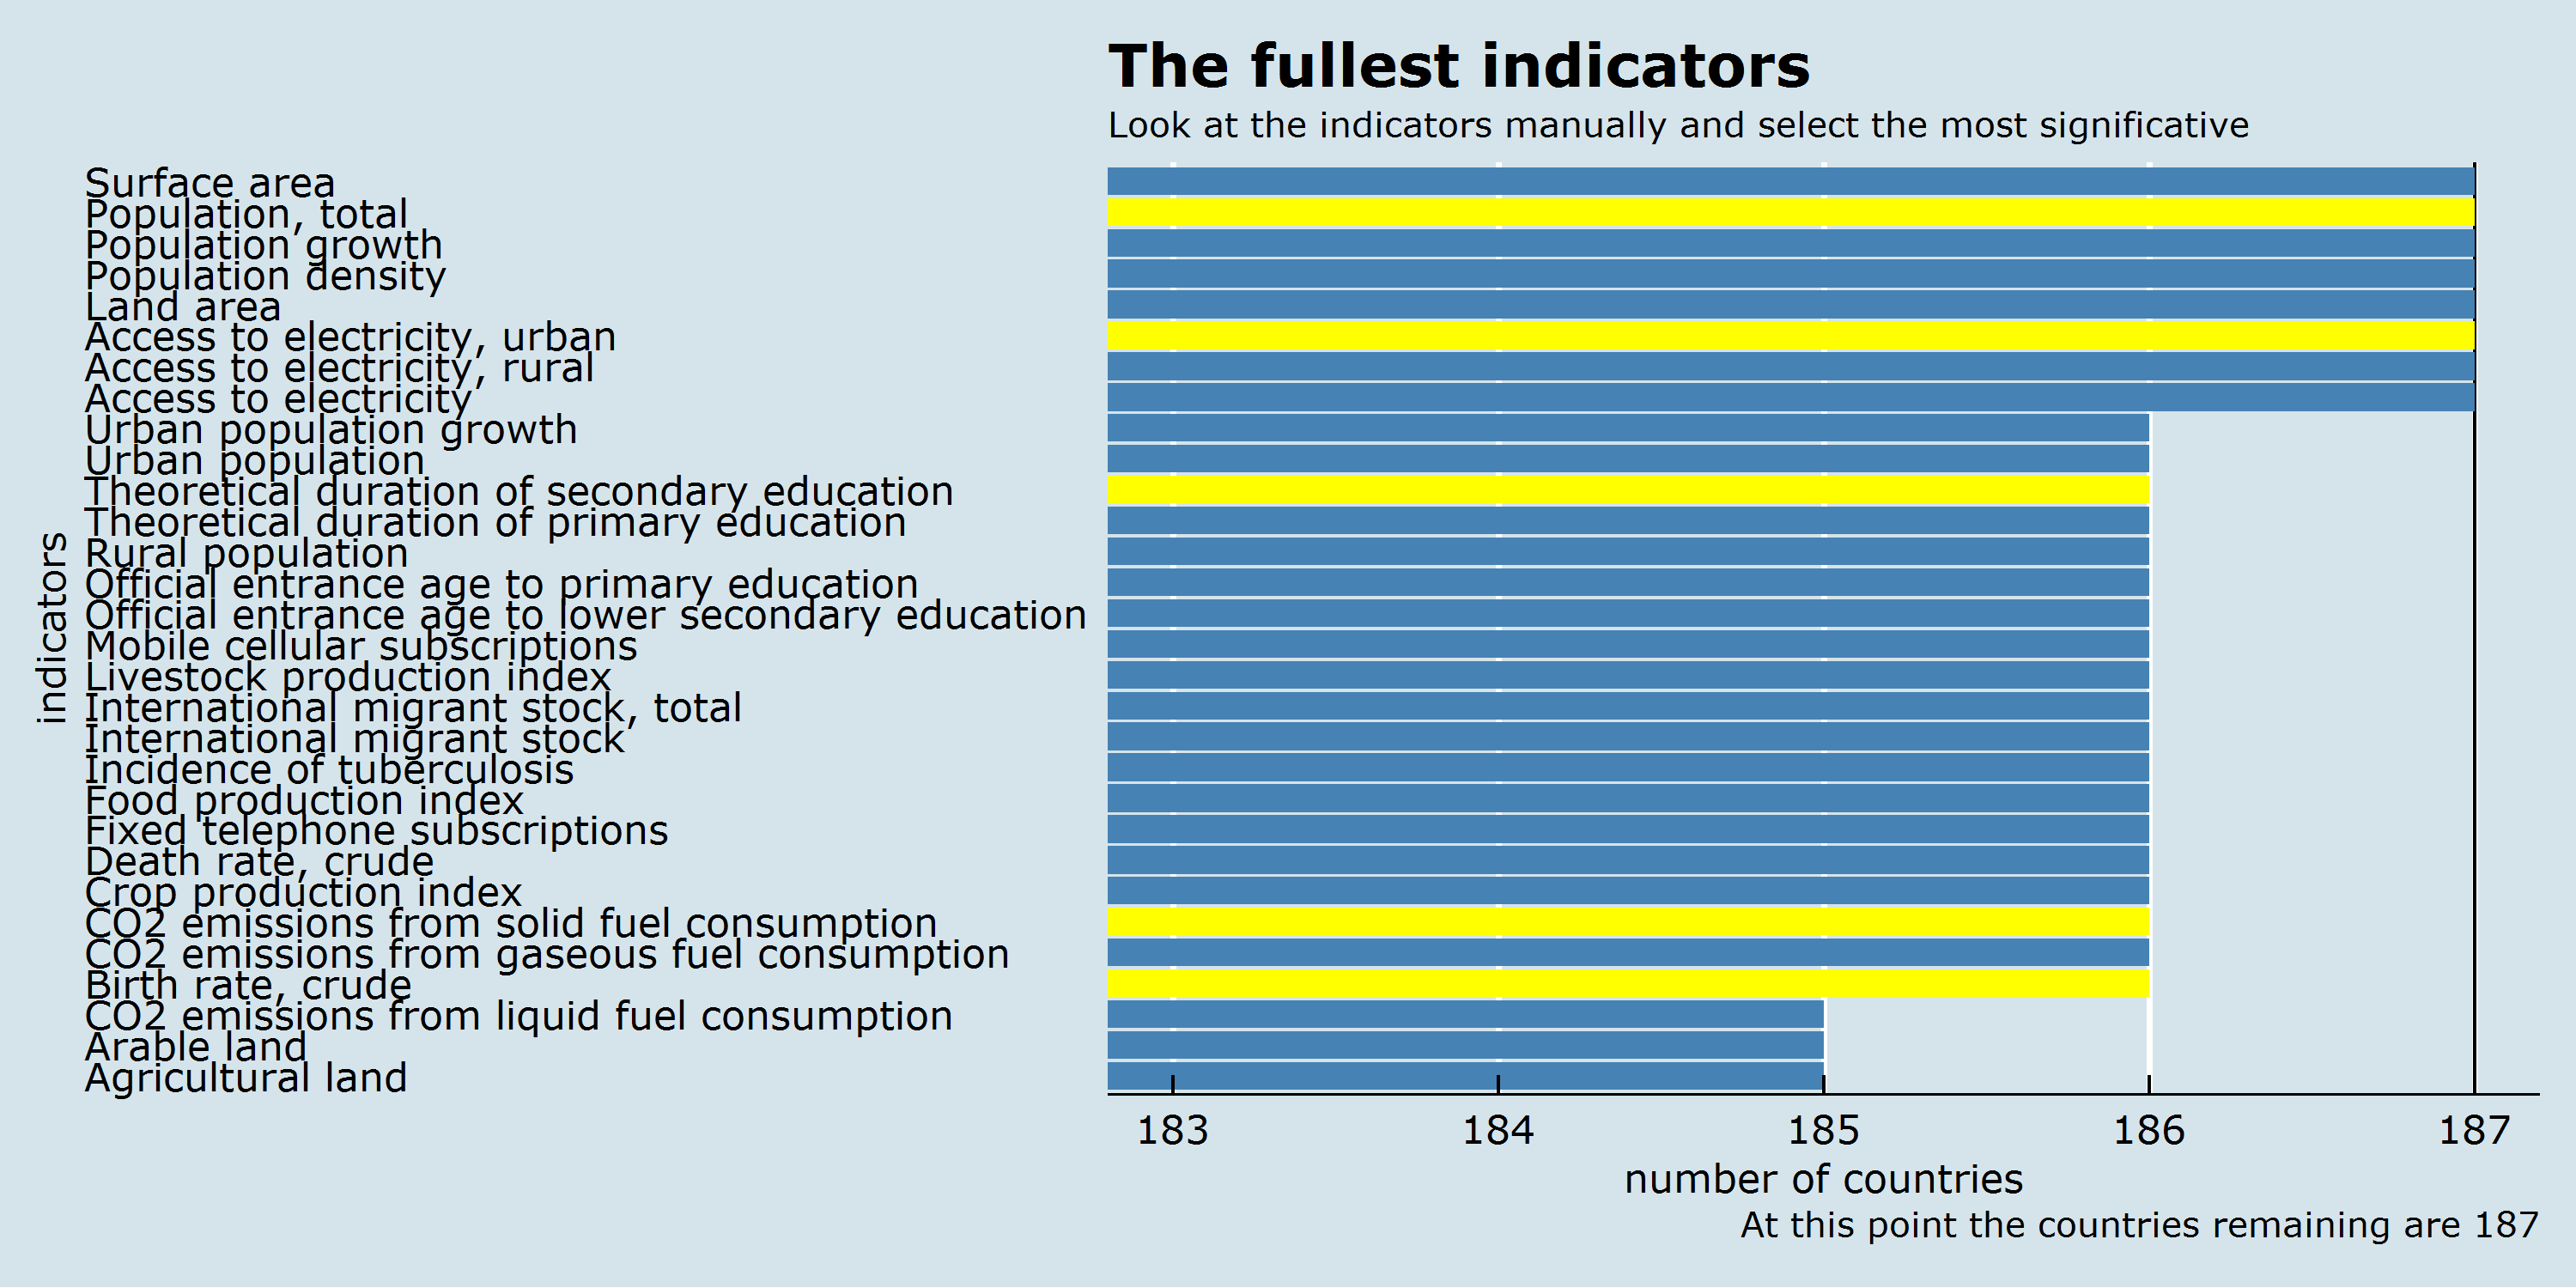
\includegraphics[width=\textwidth]{plot0007.png}
	\end{figure}
\end{frame}


% some examples of our indicators
\begin{frame}{Example 1}
	\begin{figure}
		\centering
		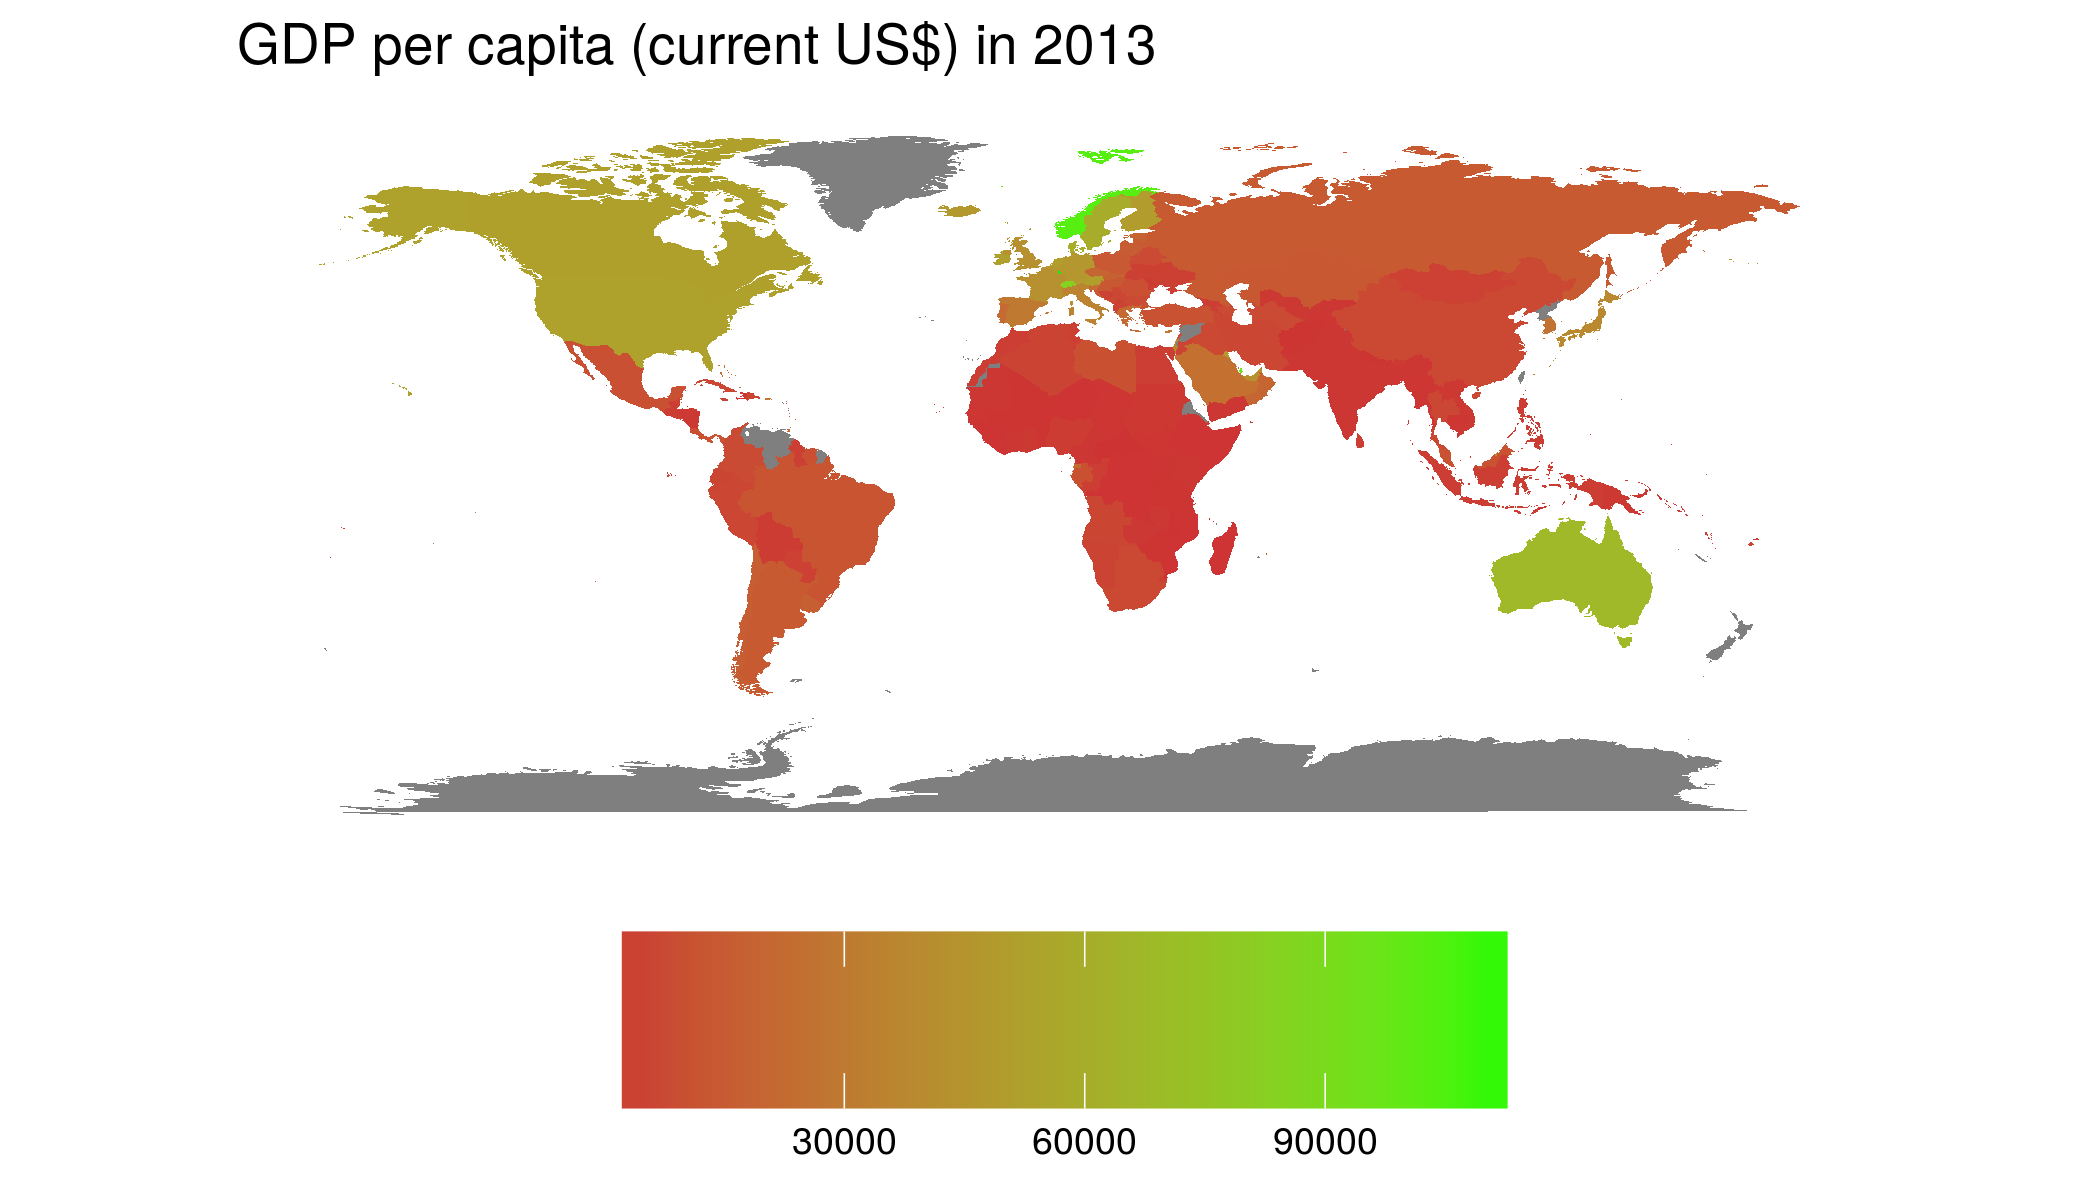
\includegraphics[width=\textwidth]{GDP.png}
		\caption[GDP per capita, 2013]{GDP per capita, 2013}
	\end{figure}
		
\end{frame}
\begin{frame}{Example 2}
	\begin{figure}
		\centering
		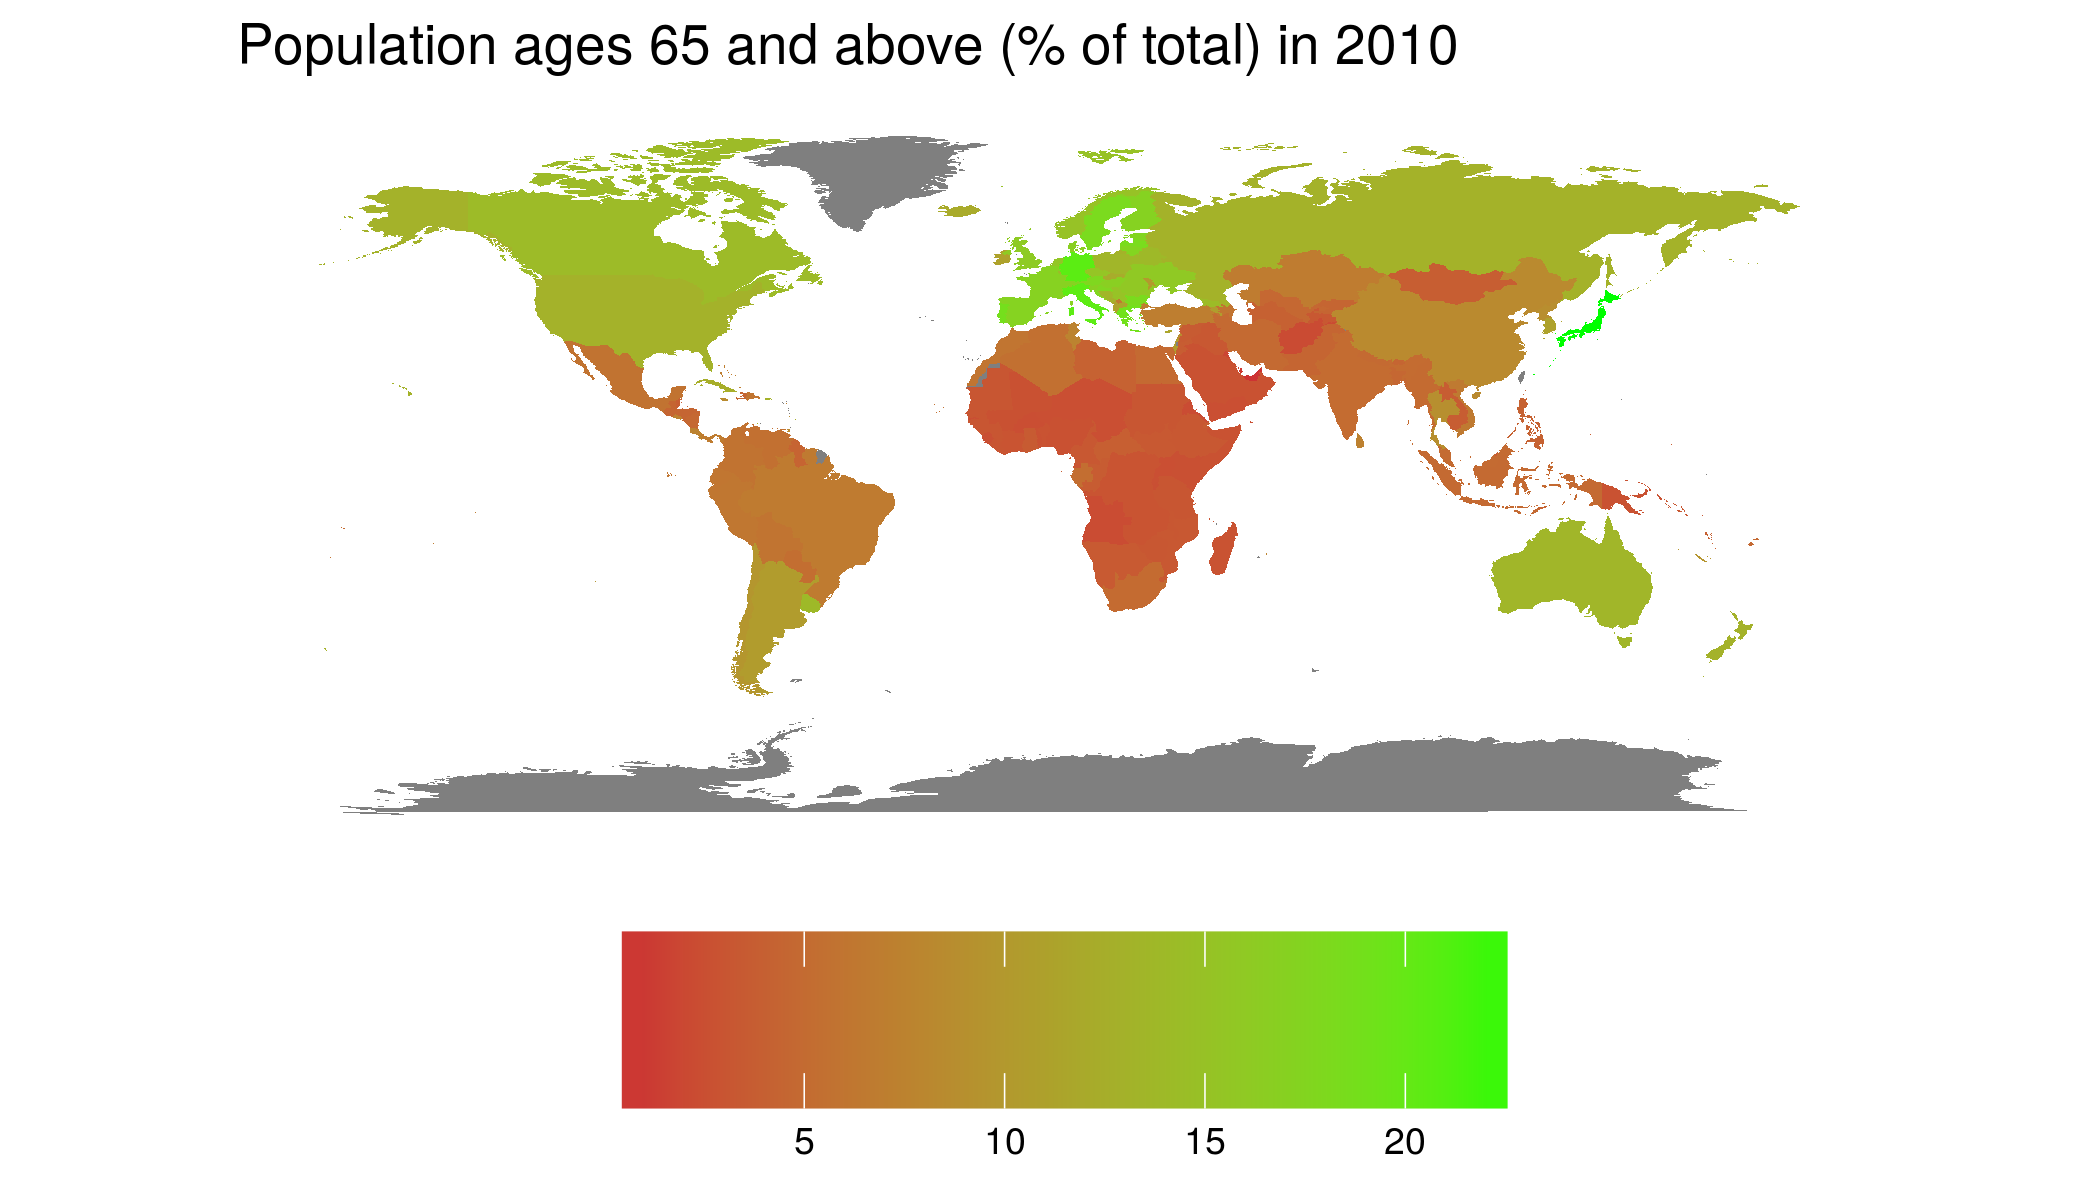
\includegraphics[width=1\textwidth]{ageing.png}
		\caption[Population aged over 65]{Population aged over 65}
	\end{figure}
\end{frame}

\begin{frame}{Example 3}
	\begin{figure}
		\centering
		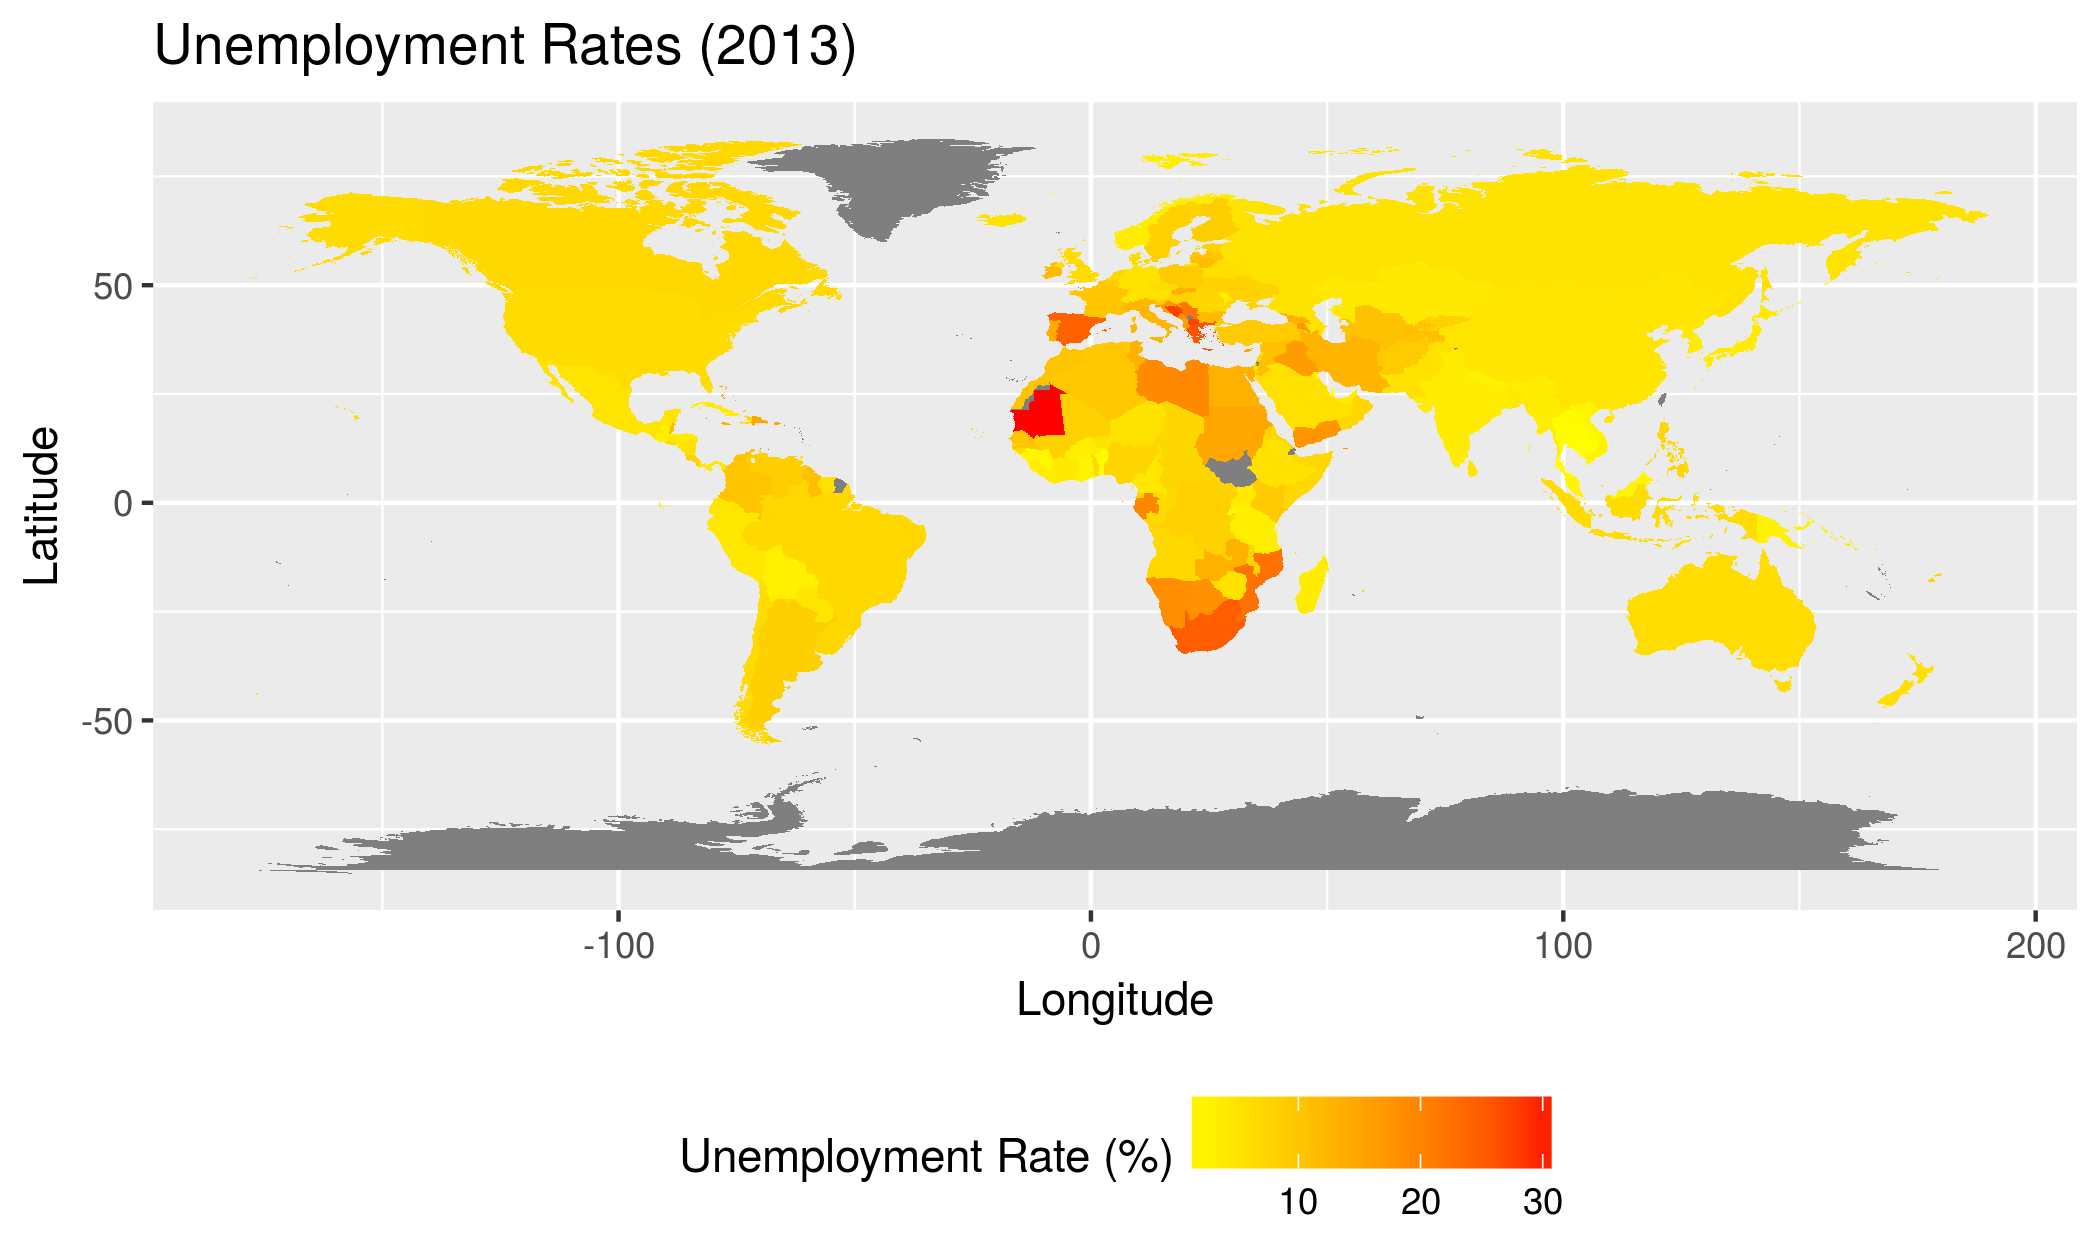
\includegraphics[width=\textwidth]{unemploy.png}
		\caption[World unemployment]{World unemployment}
	\end{figure}
\end{frame}












\end{document}